\section{A background on \acs*{WCA}}\label{sec:background}

\begin{figure}
    \centering
    \begin{subfigure}{\columnwidth}
        \centering
        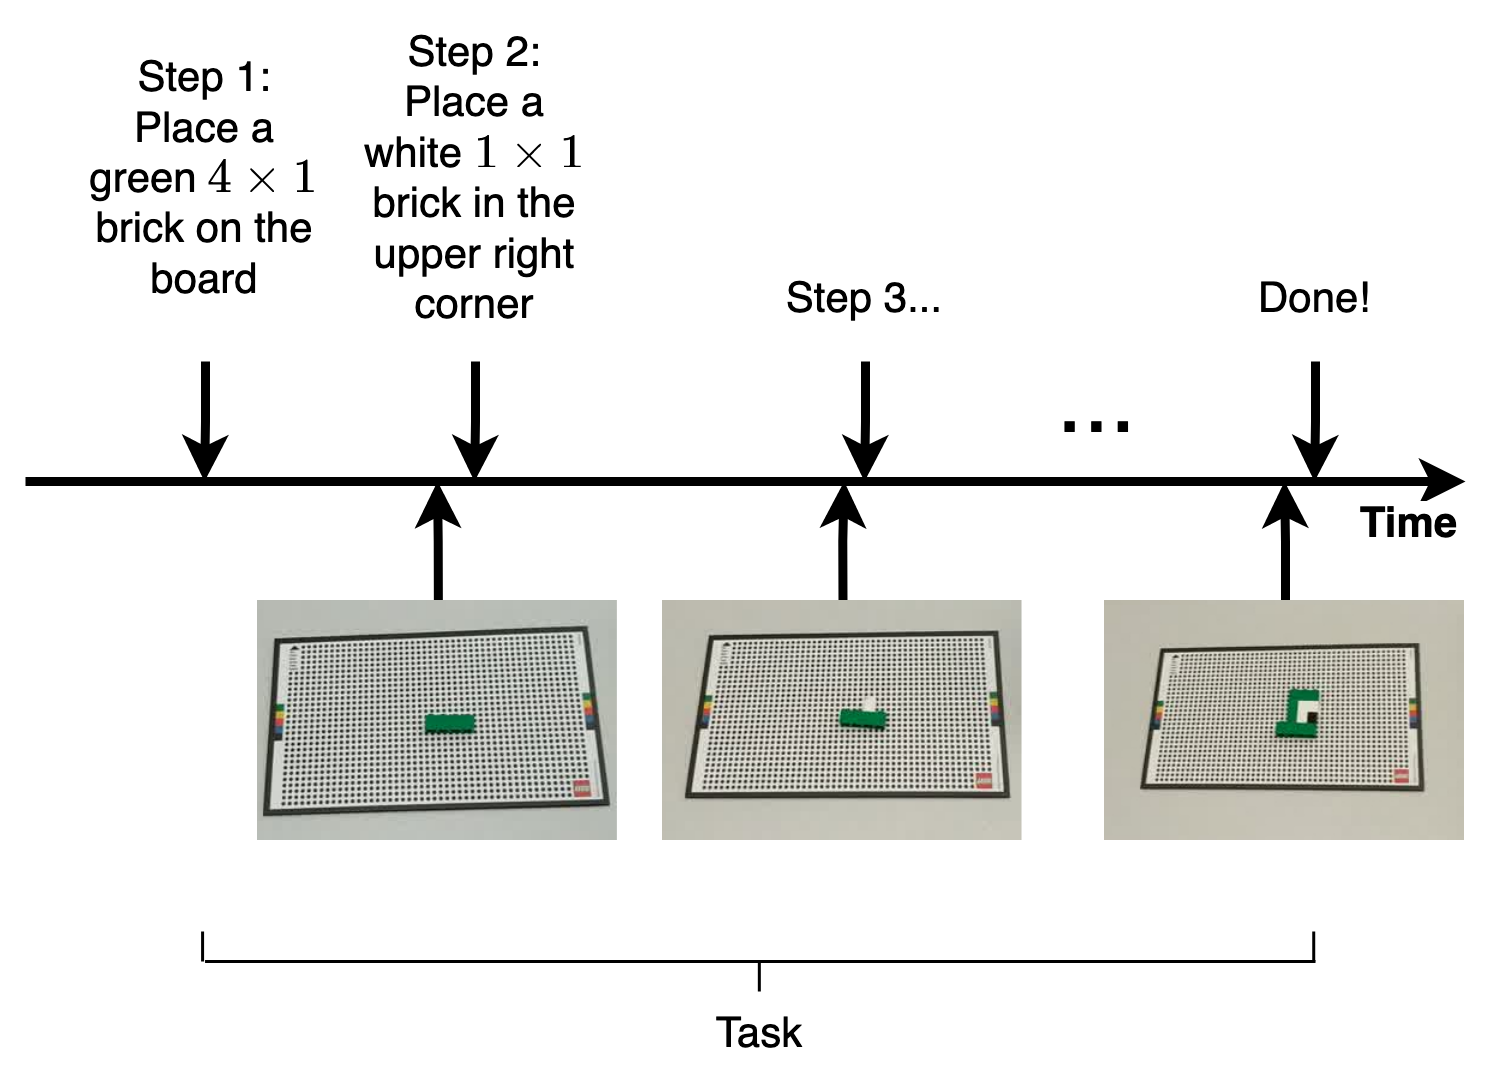
\includegraphics[width=\columnwidth]{figs/task.png}
        \caption{%
            Overview of a task in a \ac{WCA}, composed of a series of steps.
            Each steps starts with an instruction being provided to the user and ends with the instruction for the next step.
            The \ac{WCA} continuously samples the task state, automatically triggering transitions between steps as correct (or incorrect) states are recognized.
        }\label{fig:task}
    \end{subfigure}\\
    \begin{subfigure}{\columnwidth}
        \centering
        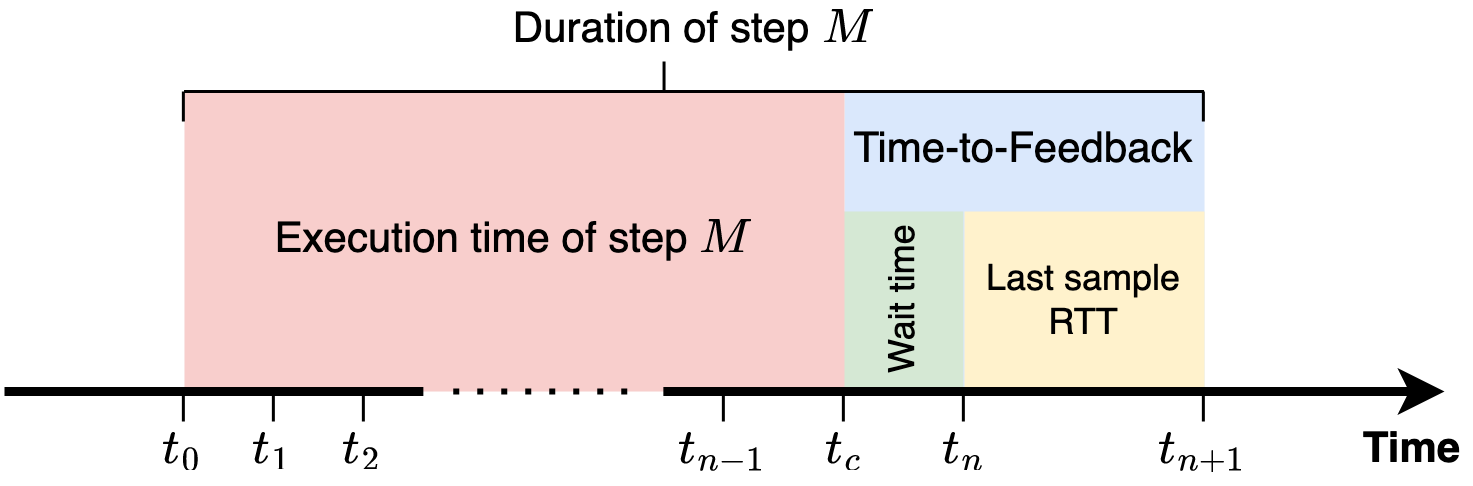
\includegraphics[width=\columnwidth]{figs/step_time.png}
        \caption{%
            Breakdown of a step into its timing components.
            The instruction for step \( M \) and \( M + 1 \) are provided to the user at \( t_0 \) and \( t_{n+1} \), respectively.
            \( t_k | k \in \{1, \ldots, n \} \) correspond to the \ac{WCA} sampling instants for step \( M \), and \( t_c \) marks the instant at which the user finishes performing the instruction.
        }\label{fig:step}
    \end{subfigure}
    \caption{}
\end{figure}

\acf{WCA} applications represent a category of novel, context-sensitive and highly-interactive \ac{AR} applications.
In this work we focus on a particular category of these applications --- denoted ``step-based'' \ac{WCA} --- which have as their ultimate goal the guiding of a user through a sequential task.
Examples of such applications are the LEGO and IKEA assistants~\cite{Chen2015LEGO,Chen2018application}, in which users are guided step-by-step through the process of assembling a LEGO model and an IKEA lamp, respectively.

Step-based \acp{WCA} operate analogously to how \ac{GPS} navigation assistants guide users, by seamlessly and continuously monitoring the progress of the user and autonomously providing relevant instructions and feedback.
The application follows the progress of the task in ``realtime'' by repeatedly sampling the state of the physical system, most commonly through video frames.
Whenever the assistant application detects that the user has correctly or incorrectly performed an instruction, it provides a new instruction to either advance the task or correct the detected mistake.
The application otherwise remains silent and out-of-the-way of the user; that is, samples which do not generate a new instruction (e.g. because they captured an intermediate or unfinished state, or simply noise) are silently discarded.
Herein lies one of key characteristics of these applications: the user only consciously interacts with the application whenever they finish an instruction, and thus these are the \emph{only} points in time at which they can notice changes in system responsiveness.

In order to discuss these applications with precision and fully understand them, we provide some definitions and explanations relating to their operation.
First of all, a \emph{step} is formally understood as a specific action to be performed by the user, described by a single instruction, and a \emph{task} consists of a series of steps to be executed in sequence (see \cref{fig:task}).
A step begins when the corresponding instruction is provided to the user, and ends when the instruction for the next step is provided; we call the time interval between these two events the \emph{step duration}.

Current implementations, such as those in~\cite{Chen2015LEGO,Chen2018application}, employ \emph{greedy} sampling.
In this scheme, a new sample is immediately taken as soon as an acknowledgement is received for the previous sample.
This means that the interval between these sampling instants is not necessarily constant, as it is subject to fluctuations due to resource contention on both the network and compute side.
It also has as a consequence that acknowledgements must be provided even for those samples which do not cause the generation of a new instruction --- these acknowledgements are simply used for flow control and do not generate user-noticeable feedback.

Take \( \{ t_0, t_1, \ldots, t_{n + 1} \} \) a series of discrete and sequential sampling intervals (following a greedy scheme) at which the \ac{WCA} captures the state of the physical system, as illustrated in \cref{fig:step}.
\( t_0 \) corresponds to the instant at which the instruction for step \( M \) is provided and the first sample is taken, and \( t_n \) to the instant at which the final sample (i.e. which captures the final state of step \( M \)) is taken. 
\( t_{n + 1} \) is then the instant at which the result for sample \( t_n \) is returned and the instruction for step \( M + 1 \) is provided.
If we define \( t_c \) as the point in time at which the user finishes performing the instruction for step \( M \), it must follow that (see also~\cite{olguinmunoz:impact2021})\footnote{\( U(a, b) \) represents the continuous uniform distribution in the open interval \( (a, b) \).}
\begin{align}\label{eq:tc}
    t_c &\thicksim U(t_{n - 1}, t_n)
\end{align}

We define the intervals \( t_c - t_0 \), \( t_n - t_c \), and \( t_{n + 1} - t_n \) as the \emph{execution time}, \emph{wait time}, and \emph{last sample \ac{RTT}}, respectively, of a step \( M \).
The sum of the latter two values (i.e. the interval \( t_{n + 1} - t_c \)) we call \emph{\ac{TTF}}.
Once again, refer to \cref{fig:step} for a visual breakdown of these values.

\subsection{The effects of changes in responsiveness on human behavior}\label{ssec:plos}

In~\cite{olguinmunoz:impact2021} we studied the effects of system responsiveness on human behavior in step-based \ac{WCA} through human-subject trials.
We employed a modified and instrumented version of the above-mentioned, step-based LEGO \ac{WCA} devised by \textcite{Chen2015LEGO}.
Subjects interacted with the assistant while we altered the responsiveness in realtime and captured key application and task performance metrics.
Additionally, we also employed questionnaires to evaluate key personality traits of the participants, and correlated these results to the task performance metrics collected.

For this work, we used \emph{delay} and execution time as the variables for system responsiveness and human behavior, respectively.
\emph{Delay} corresponded to a temporarily fixed time duration of the processing of each frame was padded to --- i.e. if during a series of steps delay was set to \( D \) seconds, the feedback for each frame was provided to the user at exactly \( D \) seconds after frame capture.
The correlation between this variable and execution time was then studied.
Delay, however, was merely an experimental tool, and if we consider
\begin{enumerate*}[itemjoin={{; }}, itemjoin={{; and }}]
    \item \cref{eq:tc} above
    \item that for a step subject to delay \( D \), \( t_k - t_{k - 1} = D \) for all \( k \in \{1, 2, \ldots, n\} \)
\end{enumerate*},
then it follows that, \emph{on average}, for \emph{all} steps subject to a delay \( D \):

\begin{align}\label{eq:ttf}
    \text{\emph{\ac{TTF}}} = \frac{3}{2}D
\end{align}

Ergo, we can directly re-parameterize the data from~\cite{olguinmunoz:impact2021} to use \ac{TTF} instead of delay by simply multiplying the delay value of each step by \num{1.5} without loss of accuracy.

With this in mind, we can reformulate the conclusions of this previous work as follows:
\begin{enumerate}
    \item System slow-down induces \emph{additional} behavioral slow-down which scales with the decrease in system responsiveness.
    Compared to the unimpaired case, participants were on average \SI{12}{\percent} slower when subject to a mean \ac{TTF} of \SI{2.475}{\second}, and a further \num{14} percentage points slower at a mean \ac{TTF} of \SI{4.5}{\second}.

    \item\label{item:speedup} At lower \acp{TTF}, humans get faster at performing steps as the task progresses, 
    For sequences of \num{12} steps in an unimpaired application state, humans executed the final four steps on average \SI{36}{\percent} faster than they did the first four.
    However, this effect is dampened by reduced system responsiveness, and actually inverts at the highest levels of system impairment; humans actually become progressively slower the longer they spend in a degraded system state.

    \item\label{item:remain} The effects of system slow-down on human behavior remain for a while even after system responsiveness improves.
    These effects are noticeable for at least \num{4} steps after the return to a high-responsiveness state. 
    
    \item The above effects are modulated by the Big Five~\cite{oliver:bfi1999} trait of \emph{neuroticism}, as evidenced by a \ac{PCA}.
\end{enumerate}

In the following, we employ the above insights together with the actual data collected for~\cite{olguinmunoz:impact2021} to design and build a probabilistic model of human behavior for \ac{WCA}.

\todo[inline]{Include section on neuroticism? Ask Bobby?}
